\documentclass[aspectratio=169,11pt]{beamer}

% ---------- Style ----------
\usetheme{Boadilla}
\usecolortheme{seahorse}
\setbeamertemplate{navigation symbols}{}
\setbeamertemplate{itemize items}[circle]
\setbeamertemplate{enumerate items}[default]
\setbeamertemplate{blocks}[rounded][shadow=false]
\usepackage{booktabs}
\usepackage{tabularx}
\usepackage{array}
\usepackage{tikz}
\usetikzlibrary{arrows.meta,positioning,shapes.multipart,calc}

\title[IPR 1 Decision Brief]{IPR 1 Decision Brief: Adelman, LP Theory, and Project Roadmap}
\subtitle{ISE 631 Project: Linear Programming Formulation of MDPs}
\author{Herbert Jockheck}
\date{Fall 2026}

\newcommand{\smallhead}[1]{\vspace{0.2em}\textbf{#1}\vspace{0.1em}}
\newcommand{\decision}[1]{\textcolor{blue!65!black}{\textbf{#1}}}

\begin{document}

% ---------- Slide 1 ----------
{%
\setbeamercolor{background canvas}{bg=white}
\begin{frame}[plain,t]
\noindent\fontsize{14}{16}\selectfont\textbf{IPR 1 Decision Brief}\par
\vspace{0.35em}

\fontsize{12}{14}\selectfont
\setbeamercolor{itemize item}{fg=black}
\setbeamercolor{itemize subitem}{fg=black}
\setbeamertemplate{itemize items}[circle]

\begin{center}
\fcolorbox{blue!55!black}{blue!8}{%
\begin{minipage}{0.90\textwidth}
\centering
\textbf{Purpose:} Confirm Adelman interpretation, ISE 631 course connection, and roadmap for completing project requirements.
\end{minipage}}
\end{center}

\vspace{0.45em}
\begin{columns}[T,onlytextwidth]
\column{0.34\textwidth}
\raggedright
\textbf{Requested decisions}
\begin{itemize}
    \setlength\itemsep{0em}
    \item Adelman interpretation?
    \item Right LP themes: simplex, duality, complementary slackness, reduced costs, column generation?
    \item Roadmap satisfies the project prompt?
    \item Surveillance-pricing extension?
\end{itemize}

\column{0.31\textwidth}
\raggedright
\textbf{Agenda today}
\begin{itemize}
    \setlength\itemsep{0em}
    \item Project scope and narrative
    \item Central research questions
    \item Adelman technique and LP connections
    \item Computational verification plan
    \item Roadmap to final submission
\end{itemize}

\column{0.31\textwidth}
\raggedright
\textbf{Successful IPR 1 end state}
\begin{itemize}
    \setlength\itemsep{0em}
    \item Scope and questions approved
    \item LP theory emphasis approved
    \item Verification requirements approved
    \item Surveillance-pricing guardrails approved
    \item Milestones to final submission approved
\end{itemize}
\end{columns}
\end{frame}
}

% ---------- Slide 2 ----------
\begin{frame}[t]{Project Scope: Core Assignment with Contemporary Motivation}
\small
\begin{block}{Working Project Concept}
\textbf{Core:} Understand, explain, and computationally verify Adelman's dynamic bid-price methodology through the lens of linear programming.\vspace{0.4em}

\textbf{Extension:} Investigate whether Adelman's framework can be meaningfully applied to a surveillance-pricing setting using real or realistically calibrated data.
\end{block}

\vspace{0.4em}
\begin{center}
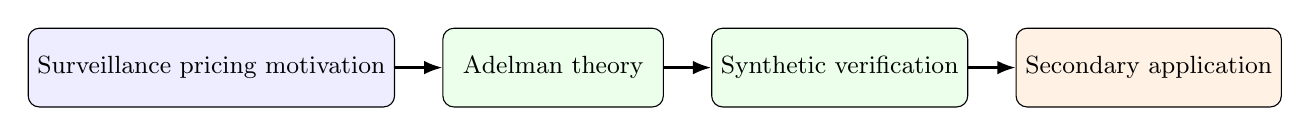
\begin{tikzpicture}[node distance=0.6cm, every node/.style={font=\small}, >=Latex]
\node[draw, rounded corners, align=center, minimum width=2.8cm, minimum height=1cm, fill=blue!7] (mot) {Surveillance\ pricing\ motivation};
\node[draw, rounded corners, align=center, minimum width=2.8cm, minimum height=1cm, fill=green!8, right=of mot] (theory) {Adelman\ theory};
\node[draw, rounded corners, align=center, minimum width=2.8cm, minimum height=1cm, fill=green!8, right=of theory] (verify) {Synthetic\ verification};
\node[draw, rounded corners, align=center, minimum width=2.8cm, minimum height=1cm, fill=orange!10, right=of verify] (apply) {Secondary\ application};
\draw[->, thick] (mot) -- (theory);
\draw[->, thick] (theory) -- (verify);
\draw[->, thick] (verify) -- (apply);
\end{tikzpicture}
\end{center}

\vspace{0.4em}
\begin{block}{Scope Guardrail}
Core project success does \textbf{not} depend on obtaining ideal surveillance-pricing data. If the application is infeasible, the completed project remains: Adelman explanation, LP-theory connection, computational verification, and critique.
\end{block}
\end{frame}

% ---------- Slide 3 ----------
\begin{frame}[t]{Approved Central Research Questions}
\small
\begin{enumerate}
    \item What is gained---and lost---by replacing the exact MDP value function with Adelman's approximate value function?
    \item Why does Adelman's approximate LP produce a bound that dominates the deterministic/fluid formulation?
    \item How do LP duality, reduced costs, and column generation make the resulting large-scale problem computationally tractable?
    \item How does the method scale with increasing state/action-space complexity, and can portions of the problem be truncated without materially changing the solution?
    \item How large are the performance gaps among the fluid formulation, approximate LP, dynamic bid-price policy, and exact MDP---and under what conditions do dynamic prices provide the greatest benefit?
    \item Can Adelman's framework be meaningfully applied to a surveillance-pricing problem using real or realistically calibrated data?
\end{enumerate}

\vspace{0.3em}
\begin{block}{IPR 1 Decision}
Are these the right organizing questions for the final paper and presentation?
\end{block}
\end{frame}

% ---------- Slide 4 ----------
\begin{frame}[t]{Adelman's Technique: What I Need to Explain Correctly}
\small
\begin{columns}[T,onlytextwidth]
\column{0.47\textwidth}
\begin{block}{Exact MDP LP}
\begin{itemize}
    \item State includes remaining time and capacity vector.
    \item Bellman inequalities create an LP over value functions.
    \item Exact formulation is theoretically clean but computationally intractable at scale.
\end{itemize}
\end{block}

\begin{block}{Approximate LP}
\begin{itemize}
    \item Replace exact value function with structured affine approximation.
    \item Preserve marginal value logic while reducing representational burden.
    \item Produces dynamic bid prices that vary with time and inventory.
\end{itemize}
\end{block}

\column{0.49\textwidth}
\begin{block}{Policy Logic}
\begin{itemize}
    \item Resource capacity has opportunity cost.
    \item Bid prices approximate marginal value of remaining capacity.
    \item Accept request when revenue exceeds implied resource opportunity cost.
\end{itemize}
\end{block}

\begin{block}{Professor Feedback Needed}
\begin{itemize}
    \item Which proof/result must I understand deeply?
    \item What level of derivation is expected in final brief?
    \item What is sufficient for ``verification'' versus full reproduction?
\end{itemize}
\end{block}
\end{columns}
\end{frame}

% ---------- Slide 5 ----------
\begin{frame}[t]{Connection to ISE 631: LP Themes to Emphasize}
\small
\begin{tabularx}{\textwidth}{>{\bfseries}p{0.25\textwidth} X}
\toprule
Course Theme & Planned Connection to Adelman \\
\midrule
Primal/dual LP & Exact MDP LP has value-function variables; dual variables can be interpreted as state-action occupancy or resource valuation. \\
\addlinespace
Complementary slackness & Links optimal policies to active constraints/support of the dual solution. \\
\addlinespace
Shadow prices & Bid prices are operational interpretations of marginal resource values. \\
\addlinespace
Simplex/reduced costs & Pricing logic asks whether omitted variables/constraints can improve or violate current solution. \\
\addlinespace
Column generation & Solves a restricted problem, uses dual information to find violated constraints or improving columns, and iterates. \\
\addlinespace
Approximation & Replaces exact, intractable LP with structured value-function approximation while preserving decision-relevant marginal values. \\
\bottomrule
\end{tabularx}

\vspace{0.4em}
\begin{block}{IPR 1 Discussion Question}
Is reduced-cost/simplex logic the right bridge for explaining Adelman's pricing/separation procedure in course language?
\end{block}
\end{frame}

% ---------- Slide 6 ----------
\begin{frame}[t]{Glidepath: Deliverables by IPR}
\small
\begin{center}
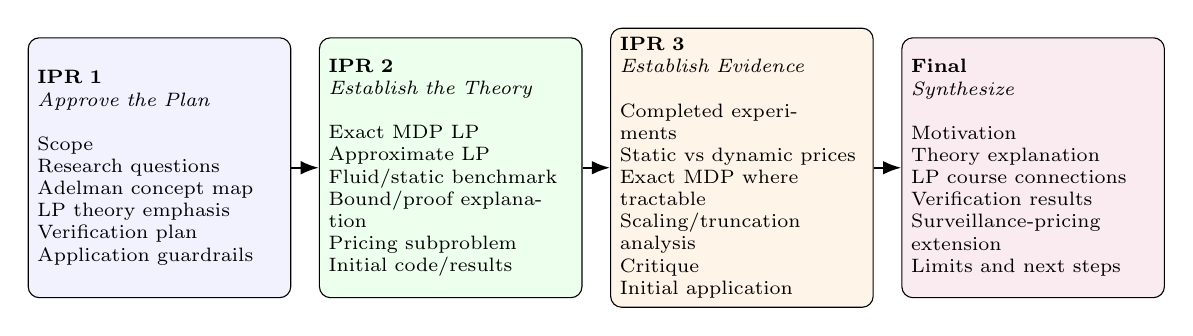
\begin{tikzpicture}[
    box/.style={draw, rounded corners, align=left, text width=3.1cm, minimum height=3.3cm, fill=blue!5, font=\scriptsize},
    >=Latex
]
\node[box] (ipr1) {\textbf{IPR 1}\newline \textit{Approve the Plan}\newline\newline
$\square$ Scope\newline
$\square$ Research questions\newline
$\square$ Adelman concept map\newline
$\square$ LP theory emphasis\newline
$\square$ Verification plan\newline
$\square$ Application guardrails};
\node[box, right=0.35cm of ipr1, fill=green!7] (ipr2) {\textbf{IPR 2}\newline \textit{Establish the Theory}\newline\newline
$\square$ Exact MDP LP\newline
$\square$ Approximate LP\newline
$\square$ Fluid/static benchmark\newline
$\square$ Bound/proof explanation\newline
$\square$ Pricing subproblem\newline
$\square$ Initial code/results};
\node[box, right=0.35cm of ipr2, fill=orange!9] (ipr3) {\textbf{IPR 3}\newline \textit{Establish Evidence}\newline\newline
$\square$ Completed experiments\newline
$\square$ Static vs dynamic prices\newline
$\square$ Exact MDP where tractable\newline
$\square$ Scaling/truncation analysis\newline
$\square$ Critique\newline
$\square$ Initial application};
\node[box, right=0.35cm of ipr3, fill=purple!8] (final) {\textbf{Final}\newline \textit{Synthesize}\newline\newline
$\square$ Motivation\newline
$\square$ Theory explanation\newline
$\square$ LP course connections\newline
$\square$ Verification results\newline
$\square$ Surveillance-pricing extension\newline
$\square$ Limits and next steps};
\draw[->, thick] (ipr1) -- (ipr2);
\draw[->, thick] (ipr2) -- (ipr3);
\draw[->, thick] (ipr3) -- (final);
\end{tikzpicture}
\end{center}
\end{frame}

% ---------- Slide 7 ----------
\begin{frame}[t]{Computational Verification and Application Plan}
\small
\begin{columns}[T,onlytextwidth]
\column{0.49\textwidth}
\begin{block}{Verification Plan}
Compare performance across synthetic instances:
\begin{itemize}
    \item deterministic/fluid formulation;
    \item static bid-price policy;
    \item Adelman dynamic bid-price policy;
    \item exact MDP solution where tractable.
\end{itemize}
Vary capacity tightness, demand uncertainty, resource/product complexity, and horizon length.
\end{block}

\begin{block}{Measures of Interest}
\begin{itemize}
    \item objective-value gaps;
    \item policy performance;
    \item computation time;
    \item sensitivity to truncation or restricted constraints.
\end{itemize}
\end{block}

\column{0.49\textwidth}
\begin{block}{Surveillance-Pricing Extension}
Feasibility test: can the application be framed as sequential decision-making under scarce resources and uncertain future demand?
\begin{itemize}
    \item state;
    \item action;
    \item reward/revenue;
    \item capacity/resource constraint;
    \item demand model;
    \item transition logic.
\end{itemize}
\end{block}

\begin{block}{Close IPR 1 With These Decisions}
Confirm project questions, theory emphasis, verification requirements, extension scope, and next deliverables for IPR 2.
\end{block}
\end{columns}
\end{frame}

\end{document}
